\chapter{基于频率特性的校正}
\section{串联超前校正}

\subsection{超前环节的性质}
超前校正环节具有如下的性质：
\begin{enumerate}
    \item 传递函数：$G_c(s) = \frac{\tau s + 1}{T s + 1} \quad \tau > T$
    \item 频率特性：$G_c(j\omega) = \frac{j\tau \omega + 1}{jT\omega + 1}$
    \item 相频特性：$\varphi (\omega) = \angle G_c(j\omega) = \arctan \tau \omega - \arctan T \omega$
    \item 幅频特性：$\left\lvert G_c(j\omega) \right\rvert = \frac{\sqrt{\tau^2 \omega^2 + 1}}{\sqrt{T^2 \omega^2 + 1}} $
    \item 最大相角对应的频率在转折频率的中点，即：$\omega_m = \frac{1}{\sqrt{T\tau}}$，此时相角：$\varphi_m = \arctan \frac{\tau - T}{2\sqrt{T \tau}}$\\
    若假设$\tau = \alpha T$，则有：$\omega_m = \frac{1}{T\sqrt{\alpha}}, \quad  \varphi_m = \arctan \frac{\alpha - 1}{2\sqrt{\alpha}} = \arcsin \frac{\alpha - 1}{\alpha + 1} $，当相角取最大时对应的幅频特性：$L_c(\omega_m) = 20 \lg \frac{\tau}{T \sqrt{\alpha}} = 10\lg \alpha$，示意图如下：

    \begin{center}
        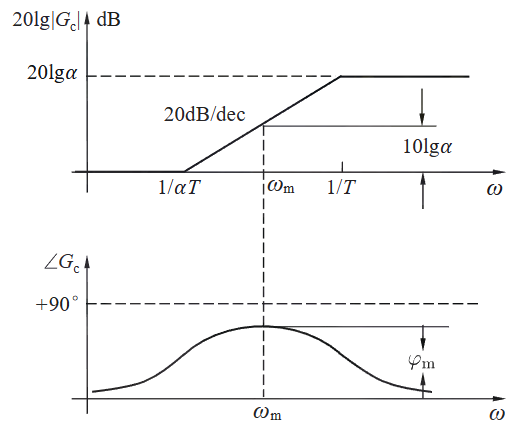
\includegraphics[width = .4\textwidth]{note/frequency correction/figure/1.png}
    \end{center}
\end{enumerate}

\subsection{单级超前校正的设计流程}

\subsubsection{相角裕度优先超前校正设计}
我们通过以下的步骤，以相角裕度要求优先为原则设计：
\begin{enumerate}
    \item 根据所要求的稳态性能指标确定系统的开环增益
    \item 利用已知的开环增益，绘制原系统的Bode图，并计算未校正系统的剪切频率$\omega_{c0}$，相角裕度$\gamma_0$
    \item 根据相角裕度的要求确定超前校正环节的$\alpha$，为使相角裕度达到要求值，计算所需增加的超前相角$\varphi_m$，即
    \begin{equation*}
        \varphi_m = \gamma - \gamma_0 + \Delta
    \end{equation*}
    上式中$\gamma$为要求的相角裕度，$\Delta$是因为考虑到校正装置影响剪切频率的位置而附加的相角，一般取$\Delta = 5\text{°} \sim  10 \text{°}$，然后根据下面这个式子计算出$\alpha$：
    \begin{equation*}
        \alpha = \frac{1+\sin \varphi_m}{1-\sin \varphi_m}
    \end{equation*}
    \item 确定校正后的系统的剪切频率$\omega_c$，在校正后的剪切频率处，未校正系统的负幅值由超前校正环节补偿，因此校正后系统的剪切频率$\omega_c$由以下的式子确定：
    \begin{equation*}
        20 \lg \left\lvert G_0(\omega_c) \right\rvert = -10 \lg \alpha
    \end{equation*}
    如果此时求得的剪切频率满足设计要求，则进行下一步；否则返回第三步调整$\Delta$
    \item 确定超前校正环节，让超前矫正环节取得最大值的频率对准校正后系统的剪切频率，即$\omega_m = \omega_c$，根据以下的式子：
    \begin{equation*}
        T = \frac{1}{\omega_m \sqrt{\alpha}}
    \end{equation*}
    确定校正装置的实践常数，进而确定校正环节的传递函数
    \item 检验系统的性能指标，若不满足要求，回到第三步重新取$\Delta$
\end{enumerate}

\subsubsection{剪切频率优先超前校正设计流程}
我们通过以下的步骤，以剪切频率要求优先为原则设计：
\begin{enumerate}
    \item 根据所要求的稳态性能指标确定系统的开环增益
    \item 利用已知的开环增益，绘制原系统的Bode图，并计算未校正系统的剪切频率$\omega_{c0}$，相角裕度$\gamma_0$
    \item 根据设计要求确定校正后系统的剪切频率$\omega_c$，并让超前校正环节取最大相角的频率对准该剪切频率，即$\omega_m = \omega_c$
    \item 根据幅值补偿确定超前校正环节的$\alpha$，在校正后的剪切频率处，未校正系统的负幅值由超前校正环节补偿，因此校正后系统的剪切频率$\omega_c$由以下的式子确定：
    \begin{equation*}
        20 \lg \left\lvert G_0(\omega_c) \right\rvert = -10 \lg \alpha
    \end{equation*}
    根据上式确定$\alpha$，按照下面的式子计算$\varphi_m$：
    \begin{equation*}
        \varphi_m = \arcsin \frac{\alpha - 1}{\alpha + 1} 
    \end{equation*}
    如果$\varphi_m = \gamma - \gamma_0 + \Delta$，$\Delta = 5\text{°} \sim  10 \text{°}$，则进行下一步，否则，返回第三步重新选择剪切频率
    \item 确定超前校正环节，由第三步和第四步确定的$\omega_m$和$\alpha$，根据以下的式子：
    \begin{equation*}
        T = \frac{1}{\omega_m \sqrt{\alpha}}
    \end{equation*}
    确定校正装置的实践常数，进而确定校正环节的传递函数
    \item 检验系统的性能指标，若不满足要求，回到第三步重新取剪切频率
\end{enumerate}

\subsubsection{相角裕度优先超前校正修正设计}
传统的相角裕度优先设计可能取不到特别合适的$\varphi_m$，所以我们通过以下的步骤，修正上述的流程
\begin{enumerate}
    \item 根据所要求的稳态性能指标确定系统的开环增益
    \item 利用已知的开环增益，绘制原系统的Bode图，并计算未校正系统的剪切频率$\omega_{c0}$，相角裕度$\gamma_0$
    \item 根据相角裕度的要求确定超前校正环节的$\alpha$，为使相角裕度达到要求值，计算所需增加的超前相角$\varphi_m$，即
    \begin{equation*}
        \varphi_m = \gamma - \gamma_0(\omega_{cL})
    \end{equation*}
    上式中$\gamma$为要求的相角裕度，$\gamma_0(\omega)$为未校正系统在$\omega$处的相位储备，$\omega_{cL}$为所要求的剪切频率的下界，根据$\varphi_m$和$\alpha$之间的关系计算出$\alpha$
    \item 确定校正后的系统的剪切频率$\omega_c$，在校正后的剪切频率处，未校正系统的负幅值由超前校正环节补偿，因此校正后系统的剪切频率$\omega_c$由以下的式子确定：
    \begin{equation*}
        20 \lg \left\lvert G_0(\omega_c) \right\rvert = -10 \lg \alpha
    \end{equation*}
    如果此时求得的剪切频率满足设计要求，则进行下一步；否则返回第三步调整$\varphi_m$
    \item 确定超前校正环节，让超前矫正环节取得最大值的频率对准校正后系统的剪切频率，即$\omega_m = \omega_c$，根据以下的式子：
    \begin{equation*}
        T = \frac{1}{\omega_m \sqrt{\alpha}}
    \end{equation*}
    确定校正装置的实践常数，进而确定校正环节的传递函数
    \item 检验系统的性能指标，若不满足要求，回到第三步重新取$\varphi_m$
\end{enumerate}

\subsection{多级超前校正设计流程}
多级超前校正设计流程可以转化为多个单级超前校正设计，后一级的超前校正以前一级超前校正的结果为条件，最后计算出的结果满足条件即可。

\textbf{注意：}如果出现$\omega_r$和$M_r$为题设要求的题要将题设条件转化为$\gamma$和$\omega_c$的条件，其中$\omega_c$的计算就是将系统强行等效为一个二阶系统，利用二阶系统的$\omega_c$与$\omega_r$之间的关系进行求解

\section{串联迟后校正}

\subsection{迟后校正环节的性质}
迟后校正环节具有如下性质：
\begin{enumerate}
    \item 传递函数：$G_c(s) = \frac{\tau s + 1}{\beta \tau s + 1}, \quad \beta > 1$
    \item 频率特性：$G_c(j\omega) = \frac{j\tau \omega + 1}{j \beta \tau \omega + 1},\quad \beta > 1$
    \item 相频特性：$\varphi(\omega) = \angle G_c(j\omega) = \arctan \tau \omega - \arctan \beta \tau \omega$
    \item 幅频特性：$\left\lvert G_c(j\omega) \right\rvert = \frac{\sqrt{\tau^2 \omega^2 + 1}}{\sqrt{\beta^2 \tau^2 \omega^2 + 1}} $
    \item 迟后校正环节的最小相角对应的频率在转折频率的中点，即：$\omega_m = \frac{1}{\tau\sqrt{\beta}}$，且有：$\varphi_m = \arctan \frac{1 - \beta}{2\sqrt{\beta}}$，具体示意图如下：
    \begin{center}
        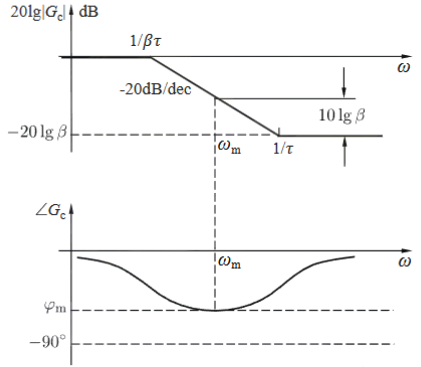
\includegraphics[width = .4\textwidth]{note/frequency correction/figure/2.png}
    \end{center}
\end{enumerate}

\subsection{单级串联迟后校正环节设计流程}

\subsubsection{相位裕度优先迟后校正设计}
我们通过以下的步骤，以相角裕度要求优先为原则设计：
\begin{enumerate}
    \item 按稳态性能的要求确定系统的型别和开环增益
    \item 利用已知的开环增益，绘制未校正系统$G_0(j\omega)$的Bode图，并计算未校正系统的剪切频率$\omega_{c0}$和相角裕度$\gamma_0$
    \item 确认校正后系统的剪切频率$\omega_c$，该剪切频率应该满足下式：
    \begin{equation*}
        180\text{°}+ \angle G_0(j\omega_c) = \gamma + \Delta
    \end{equation*}
    其中$\gamma$为要求的相角裕度，$\Delta$是由于校正装置产生的相位迟后效应而附加的相角
    \item 确定校正装置的$\beta$值，为使校正后的系统在剪切频率出幅频特性为0dB，应有：
    \begin{equation*}
        20 \lg \left\lvert G_0(j\omega_c) \right\rvert - 20\lg \beta = 0 
    \end{equation*}
    即
    \begin{equation*}
        \beta = \left\lvert G_0(j\omega_c) \right\rvert 
    \end{equation*}
    \item 确定迟后校正环节的参数$\tau$，为减小串联迟后校正对系统相位裕度的影响，要求矫正环节在剪切频率$\omega_c$处的迟后相移在6°$\sim$12°以下，应当选择：
    \begin{equation*}
        \tau = (5 \sim 10) \frac{1}{\omega_c}
    \end{equation*}
    \item 校验校正后系统的相位裕度和其余性能指标，如不满足要求，返回第三步重新选择$\Delta$，直到满足要求
\end{enumerate}

\subsubsection{剪切频率优先迟后校正设计}
我们通过以下的步骤，以剪切频率要求优先为原则设计：
\begin{enumerate}
    \item 按稳态性能的要求确定系统的型别和开环增益
    \item 利用已知的开环增益，绘制未校正系统$G_0(j\omega)$的Bode图，并计算未校正系统的剪切频率$\omega_{c0}$和相角裕度$\gamma_0$
    \item 确认校正后系统的剪切频率$\omega_c$，该剪切频率应该满足下式：
    \begin{equation*}
        180\text{°}+ \angle G_0(j\omega_c) > \gamma + \Delta
    \end{equation*}
    其中$\gamma$为要求的相角裕度，$\Delta$是由于校正装置产生的相位迟后效应而附加的相角
    \item 确定校正装置的$\beta$值，为使校正后的系统在剪切频率出幅频特性为0dB，应有：
    \begin{equation*}
        20 \lg \left\lvert G_0(j\omega_c) \right\rvert - 20\lg \beta = 0 
    \end{equation*}
    即
    \begin{equation*}
        \beta = \left\lvert G_0(j\omega_c) \right\rvert 
    \end{equation*}
    \item 确定迟后校正环节的参数$\tau$，为减小串联迟后校正对系统相位裕度的影响，要求矫正环节在剪切频率$\omega_c$处的迟后相移在6°$\sim$12°以下，应当选择：
    \begin{equation*}
        \tau = (5 \sim 10) \frac{1}{\omega_c}
    \end{equation*}
    \item 校验校正后系统的相位裕度和其余性能指标，如不满足要求，返回第三步重新选择$\Delta$，直到满足要求
\end{enumerate}

\section{串联迟后-超前校正}
在此设计方法中，迟后校正的主要作用使降低系统的剪切频率，不关注它对系统相角裕度的影响；相角裕度提高的任务交给超前校正环节

尽管如此，由于迟后校正环节降低了剪切频率，通过利用原系统的相位储备，迟后校正后系统的相角裕度事实上得到了部分提升

\subsection{迟后环节优先的迟后-超前校正环节设计}

\subsubsection{剪切频率优先设计流程}
我们通过以下的步骤，以剪切频率要求优先为原则设计：（针对超前校正而言）
\begin{enumerate}
    \item 绘制满足稳态误差要求的未校正系统开环频率特性的Bode图，由于串联超前校正可以有效增加相角裕度，所以首先\textbf{采用串联迟后校正，使系统的剪切频率满足或接近于满足设计要求}，在此基础上，再采用串联超前校正，使相角满足设计要求
    \item 考虑到进行串联超前校正时，会使原系统剪切频率增大，所以在进行串联迟后校正时可以使剪切频率略小于设计要求，使用剪切频率优先迟后校正发确定迟后校正环节
    \item 计算出串联迟后校正环节后的系统幅频特性曲线，求出剪切频率$\omega_c$和相角裕度$\gamma$
    \item 在这一步将对迟后校正后的系统进行超前校正，采用剪切频率优先超前校正法获得超前校正装置的传递函数
    \item 验证系统性能指标，如不满足要求，则回到第二步或者第四步重新设计
\end{enumerate}

\subsubsection{相角裕度优先设计流程}
我们通过以下的步骤，以剪切频率要求优先为原则设计：（针对超前校正而言）
\begin{enumerate}
    \item 绘制满足稳态误差要求的未校正系统开环频率特性的Bode图，由于串联超前校正可以有效增加相角裕度，所以首先\textbf{采用串联迟后校正，使系统的剪切频率满足或接近于满足设计要求}，在此基础上，再采用串联超前校正，使相角满足设计要求
    \item 考虑到进行串联超前校正时，会使原系统剪切频率增大，所以在进行串联迟后校正时可以使剪切频率略小于设计要求，使用剪切频率优先迟后校正发确定迟后校正环节
    \item 计算出串联迟后校正环节后的系统幅频特性曲线，求出剪切频率$\omega_c$和相角裕度$\gamma$
    \item 在这一步将对迟后校正后的系统进行超前校正，采用相角裕度优先超前校正法获得超前校正装置的传递函数
    \item 验证系统性能指标，如不满足要求，则回到第二步或者第四步重新设计
\end{enumerate}

\subsection{超前环节优先的迟后-超前校正环节设计}

\subsubsection{迟后环节提高稳态精度的超前环节优先的迟后-超前校正环节设计}

我们通过以下步骤进行校正环节的设计：（通过迟后环节提高稳态精度）
\begin{enumerate}
    \item 按稳态性能的要求确定系统的型别和开环增益$K$。利用已知的开环增益，绘制为校正系统$G_0(s)$的Bode图，并计算未校正系统的剪切频率$\omega_{c0}$，相角裕度$\gamma_0$
    \item 对$G_0(s)$仅改变开环增益，选择合适的开环增益$K_1$使得所对应的系统$G_{01}(s)$的剪切频率$\omega_{c1}$小于所要求的剪切频率$\omega_c$
    \item 对系统$G_{01}(s)$进行超前校正确定超前校正环节$G_{c1}(s)$的传递函数
    \begin{equation*}
        G_{c1}(s) = \frac{\alpha T s + 1}{Ts+1}
    \end{equation*}
    为使最终校正系统的相角裕度达到设计要求，超前环节提供的超前相角$\varphi_m$为：
    \begin{equation*}
        \varphi_m = \gamma - \gamma_{01}(\omega_{cL}) + \Delta_1 + \Delta_2
    \end{equation*}
    式中$\gamma$为所要求的相角裕度，$\gamma_{01}(\omega_{cL})$是系统$G_{01}(s)$在所要求的下限频率$\omega = \omega_{cL}$处的相位储备，$\Delta_1$是考虑到校正装置影响剪切频率的位置而附加的相角，$\Delta_2$是为了抵消迟后校正环节所产生的相位延迟而附加的相角，参数$\alpha$由下式确定
    \begin{equation*}
        \alpha = \frac{1+\sin\varphi_m}{1-\sin\varphi_m}
    \end{equation*}
    未校正系统$G_{01}(s)$的负幅值由超前校正环节补偿，因此校正后系统的剪切频率由下式确定：
    \begin{equation*}
        20 \lg \left\lvert G_{01}(j \omega_c) \right\rvert = -10 \lg \alpha
    \end{equation*}
    若得到的剪切频率不满足要求，则增大$\Delta_2$重新进行第三步操作。若仍不满足要求，返回第二步重新选择开环增益，若得到的剪切频率满足要求，则使超前校正环节的最优频率$\omega_m$位于$\omega_c$处，得到超前校正环节时间常数为$T = \frac{1}{\omega_m \sqrt{\alpha}}$
    \item 检验超前校正后的系统$G_1(s)$的动态性能，注意其相角裕度是否能补偿迟后环节的相位延迟
    \item 根据超前校正后的系统确定迟后校正环节
    \item 检验校正后的系统的性能指标，如果不满足，返回第二步
\end{enumerate}

\subsubsection{迟后环节降低剪切频率的超前环节优先的迟后-超前校正环节设计}
我们通过以下步骤进行校正环节的设计：（通过迟后环节降低剪切频率）
\begin{enumerate}
    \item 按稳态性能的要求确定系统的型别和开环增益$K$。利用已知的开环增益，绘制为校正系统$G_0(s)$的Bode图，并计算未校正系统的剪切频率$\omega_{c0}$，相角裕度$\gamma_0$
    \item 选取满足要求的剪切频率$\omega_c$，对系统$G_{0}(s)$进行超前校正确定超前校正环节$G_{c1}(s)$的传递函数
    \begin{equation*}
        G_{c1}(s) = \frac{\alpha T s + 1}{Ts+1}
    \end{equation*}
    为使最终校正系统的相角裕度达到设计要求，超前环节提供的超前相角$\varphi_m$为：
    \begin{equation*}
        \varphi_m = \gamma - \gamma_{01}(\omega_{c})  + \Delta_2
    \end{equation*}
    式中$\gamma$为所要求的相角裕度，$\gamma_{0}(\omega_{c})$是系统$G_{0}(s)$在$\omega = \omega_{c}$处的相位储备，$\Delta_2$是为了抵消迟后校正环节所产生的相位延迟而附加的相角，参数$\alpha$由下式确定
    \begin{equation*}
        \alpha = \frac{1+\sin\varphi_m}{1-\sin\varphi_m}
    \end{equation*}
    使超前校正环节的最优频率$\omega_m$位于$\omega_c$处，得到超前校正环节时间常数为
    \begin{equation*}
        T = \frac{1}{\omega_m \sqrt{\alpha}}
    \end{equation*}
    \item 检验超前校正后的系统$G_1(s)$的动态性能，注意其相角裕度是否能补偿迟后环节的相位延迟
    \item 根据超前校正后的系统确定迟后校正环节
    \item 检验校正后的系统的性能指标，如果不满足，返回第二步
\end{enumerate}

\textbf{对于以上两种方法，概括一下就是：}
\begin{enumerate}
    \item 恰当选取$\omega_c$，利用超前校正提升$\omega_c$处的相角，并使校正后的幅值>0dB，超前校正的作用主要是增大相角裕量，并保证较大的剪切频率
    \item 再利用迟后校正的幅值衰减作用使校正后的$\omega_c$处的幅值等于0dB，迟后校正的作用是使超前校正后$\omega_c$处的幅值衰减到0dB
\end{enumerate}

\section{期望频率特性法}

\subsection{控制系统的性能要求}
我们对于控制系统有以下几项性能要求：
\begin{enumerate}
    \item \textbf{对稳态误差的要求：}这项要求对应于系统开环传递函数串联积分环节数$v$和开环增益$K$
    \item \textbf{对系统超调量$\sigma_p$的要求：}这一要求对应于系统的相角裕度$\gamma$或者相对谐振峰值$M_r$。对于高阶系统，经常使用如下经验公式：
    \begin{equation*}
        \sigma_p = 0.16 + 0.4 \left(\frac{1}{\sin \gamma} - 1\right)
    \end{equation*}
    或者
    \begin{equation*}
        \sigma_p = 0.16 + 0.4 (M_r - 1)
    \end{equation*}
    \item \textbf{对系统调整时间$t_s$的要求：}根据对调整时间$t_s$和相角裕度$\gamma$的要求可以求取系统的剪切频率$\omega_c$。对于高阶系统，经常使用如下的经验公式：
    \begin{equation*}
        t_s = \frac{\pi}{\omega_c}\left[2 + 1.5\left(\frac{1}{\sin \gamma} - 1\right) + 2.5 \left(\frac{1}{\sin\gamma} - 1\right)^2 \right]
    \end{equation*}
    或者
    \begin{equation*}
        t_S = \frac{\pi}{\omega_c}\left[ 2 + 1.5(M_r - 1) + 2.5 (M_r - 1)^2 \right]
    \end{equation*}
\end{enumerate}

\subsection{对中频段的设计方法}

\subsubsection{对称最佳方法确定中频段}
我们通过以下的几个式子确定中频段：
\begin{equation*}
    \begin{split}
        \sigma_p &= 0.16 + 0.4\left(\frac{1}{\sin \gamma} - 1\right) \\
        t_s &= \frac{\pi}{\omega_c} \left[ 2 + 1.5 \left( \frac{1}{\sin \gamma} - 1\right) + 2.5 \left(\frac{1}{\sin \gamma} - 1\right)^2\right] \\ 
        h &= \frac{1 + \sin \gamma}{1-\sin\gamma} \\
        \omega_2 & \leq \frac{\omega_c}{\sqrt{h}} , \quad \omega_3 \geq \omega_c \sqrt{h}\\
    \end{split}
\end{equation*}

\subsubsection{剪切频率错位确定中频段}
我们通过以下的几个式子确定中频段：
\begin{equation*}
    \begin{split}
        \sigma_p &= 0.16 + 0.4\left(\frac{1}{\sin \gamma} - 1\right) \\
        t_s &= \frac{\pi}{\omega_c} \left[ 2 + 1.5 \left( \frac{1}{\sin \gamma} - 1\right) + 2.5 \left(\frac{1}{\sin \gamma} - 1\right)^2\right] \\ 
        h &= \frac{1 + \sin \gamma}{1-\sin\gamma} \\
        \omega_2 & \leq \omega_c \frac{2}{h+1} , \quad \omega_3 \geq \omega_c \frac{2h}{h+1}\\
    \end{split}
\end{equation*}

\subsubsection{最小峰值法确定中频段}

我们通过以下的几个式子确定中频段：
\begin{equation*}
    \begin{split}
        \sigma_p &= 0.16 + 0.4\left(M_r - 1\right) \\
        t_s &= \frac{\pi}{\omega_c} \left[ 2 + 1.5 \left( M_r - 1\right) + 2.5 \left(M_r - 1\right)^2\right] \\ 
        \omega_2 & \leq \omega_c \frac{M_r - 1}{M_r} , \quad \omega_3 \geq \omega_c \frac{M_r+1}{M_r}\\
    \end{split}
\end{equation*}

\subsection{期望频率特性法的设计步骤}

我们可以通过以下步骤，采用期望频率特性法来设计校正环节：
\begin{enumerate}
    \item 根据稳态误差确定型别$v$和开环增益$K$，并绘制未校正系统$G_0(s)$的幅频特性。期望频率特性的低频段与未校正系统低频段相同，即为：
    \begin{equation*}
        G_L(s) = \frac{K}{s^v}
    \end{equation*}
    \item 根据对系统的动态特性要求，确定期望特性中的中频段特性，包括剪切频率、上限角频率和下限角频率，并使其斜率为-20dB/dec
    \item 确定期望特性低频段和中频段的过渡特性，其斜率一般取-40dB/dec
    \item 确定期望特性的高频段特性，高频段应尽量等于或平行于校正前的高频段
    \item 确定期望特性中频段和高频段的过渡特性，其斜率一般取-40dB/dec
    \item 基于以上步骤确定期望频率特性$G(j\omega)$，并检验性能指标。如不满足要求，返回第2步重新设计
    \item 根据库期望频率特性$(G(j\omega))$和校正前的频率特性$G_0(j\omega)$确定校正装置的传递函数$G_c (s) = \frac{G(s)}{G_0(s)}$
\end{enumerate}

\section{反馈校正}

\subsection{反馈校正的功能}

反馈校正有以下几个功能：
\begin{enumerate}
    \item 改变局部结构和参数：位置反馈可以降低开环增益，速度反馈可以降低剪切频率
    \item 降低参数敏感性：通过反馈校正可以降低原本开环传递函数的变化对于输出的影响
    \item 等效串联反馈：通过设计一个简单的反馈校正可以等效一个比较复杂的串联校正
    \item 消除不希望折点：通过反馈校正可以消除一个我们不想要的转折频率，增大系统的剪切频率以满足设计指标
\end{enumerate}

\subsection{反馈校正的设计}

\subsubsection{设计理念}

假设有一个系统如下图所示，我们在中间环节加入反馈校正，使得校正后的系统满足我们的设计要求，此时校正系统的开环传递函数为：
\begin{center}
    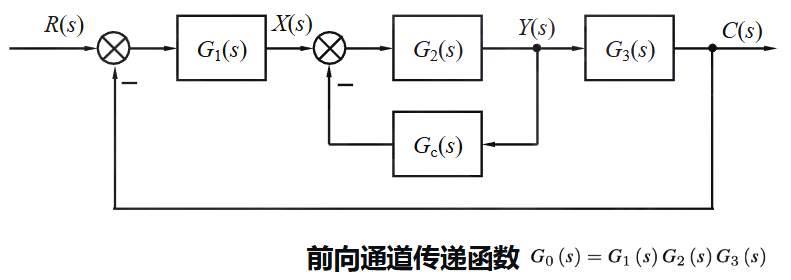
\includegraphics[width = .7\textwidth]{note/frequency correction/figure/3.png}
\end{center}

\begin{equation*}
    G(s) = \frac{G_0(s)}{1 + G_2(s) G_c(s)}
\end{equation*}
在满足$20\lg \left\lvert G_2(j\omega) G_c(j\omega) \right\rvert \ll 0$的频段，由上式可以看出此时校正系统的开环频率特性近似写为：
\begin{equation*}
    G(s) \approx G_0(s)
\end{equation*}
在满足$20\lg\left\lvert G_2(j\omega) G_c(j\omega) \right\rvert \gg 0 $的频段，由上式可以看出此时校正系统的开环频率特性近似写为
\begin{equation*}
    G(s) \approx \frac{G_0(s)}{G_2(s) G_c(s)}
\end{equation*}
这个式子可以等价写为：
\begin{equation*}
    G_2(s) G_c(s) \approx \frac{G_0(s)}{G(s)}
\end{equation*}
在反馈校正的过程中，应当注意两点：
\begin{enumerate}
    \item 在$20\lg\left\lvert G_2(j\omega) G_c(j\omega) \right\rvert > 0 $的受校正频段内，应当使$20\lg\left\lvert G_0(j\omega) \right\rvert > 20\lg\left\lvert G(j\omega) \right\rvert  $，这个式子大得越多，校正精度越高
    \item 局部反馈回路必须稳定
\end{enumerate}

\subsubsection{设计流程}

我们通过期望频率特性法来设计反馈校正：
\begin{enumerate}
    \item 按照稳态性能指标要求，绘制待校正系统的开环对数幅频特性$L_0(\omega)$
    \item 根据给定性能指标要求，绘制期望开环对数幅频特性$L(\omega)$
    \item 由下式求得$G_2(s) G_c(s)$的传递函数
    \begin{equation*}
        20 \lg \left\lvert G_2(j\omega) G_c(j\omega) \right\rvert = L_0(\omega) - L(\omega) 
    \end{equation*}
    \item 检验局部反馈回路的稳定性，并检查期望剪切频率附近$\left\lvert G_2(j\omega) G_c(j\omega) \right\rvert > 1 $的程度
    \item 由$G_2 G_c$求$G_c$
    \item 检验校正后系统的性能指标是否满足要求
\end{enumerate}